\documentclass{article}
\usepackage{hyperref}
\usepackage{float}
\usepackage{graphicx}
\usepackage{caption}
\usepackage{subcaption}
\graphicspath{{../../images/}}

\hypersetup{
    colorlinks=true,
    linkcolor=blue,
    filecolor=magenta,      
    urlcolor=cyan,
    pdftitle={Overleaf Example},
    pdfpagemode=FullScreen,
    }

\title{Graph Creation from Relations}
\author{Rajiv Sambasivan}
\date{\today}

\begin{document}

\maketitle

\section{Introduction}
Though we may not always be aware of it, the data we use for analytics or machine learning is often relational in nature. This means that the data we analyze or learn from typically consists of domain entities interacting with each other, often with a timestamp for each interaction. For example, in a retail dataset, we might have customers, products, and transactions, where each transaction links a customer to a product. Constructing a graph from such relational data can help us better understand the relationships and interactions between these entities. Operations Research (Network Models), Machine Learning (Graph Signal Processing, Graphical Models), and Data Science (Graph Analytics) all offer several canonical methods for working with graphs. The theory and practice of solving these canonical problems are well established. Creating a graph from a set of relations enables us to explore these methods and apply them to our data.  If you are working with relational data, then there is a good chance that a graph perspective can benefit your use case.

There is more to applying the above ideas than simply creating a graph from the data. In the context of machine learning, when working with large datasets, there is typically \emph{heterogeneity} in the relationships between entities. In a supervised learning setting, this may manifest in how predictors are related to each other and to the target variable. In an unsupervised learning setting, this may manifest in clustering or grouping of entities changing over time or across different subsets of the data. In a dimension reduction setting, the eigen values and eigen vectors of the covariance matrix may change across different subsets of the data and over time.

Typically, this heterogeneity can be characterized by using a small number of graphs to represent our data. Each graph has the same predictor-response relationship and the same relationships between predictors. In other words, rather than using a single graph to represent the entire dataset, we often have to use multiple graphs, each of which is homogeneous with respect to the analysis or learning task.



\section{Graph Relational Learning, not a new idea}
The idea of creating a graph from relations is not new. \cite{getoor2007introduction} is an entire textbook on the topic of graph relational learning. Applying neural networks to graphs is also not a new idea. \cite{schlichtkrull2018modeling} is a paper on the topic of applying convolutional neural networks to relational data using a graph perspective. The principal challenges to applying these ideas, in my experience, are:
\begin{itemize}
\item Identifying this pattern as a standard approach to model problems where the IID assumption does not hold. There are other approaches, such as hierarchical modeling, that can be used to model such problems, but given the availability of graph machine learning tools, it is often easier to use a graph perspective.
\item Identifying standard ways to represent the input data as relations between entities. For example, do we want to reduce the data to a single n-ary relation, or do we want to use multiple relations to represent the data?
\item Identifying the heterogeneity in the relationships between entities. What constitutes heterogeneity in the relationships between entities is application and task-dependent. The methods we use to identify heterogeneity in the relationships between entities differ in a balanced classification task (where the target variable distribution is balanced) and an unbalanced classification task (where the target variable distribution is unbalanced). The methods we use for unsupervised learning problems are different from those we use for supervised learning problems. Standardization of how the methods used to identify heterogeneity in the data by tasks, for example, for clustering, imbalanced classification, and regression, is key to applying the methods effectively. Making the type of data used for modeling - cross-sectional, time series, or spatio-temporal - explicit in the data representation provides a way to develop guidelines for how to identify heterogeneity in the relationships between entities.
\end{itemize}
Once we have created a graph from the relations and have identified the heterogeneity, there are canonical problem representations, such as node classification/regression or link prediction, that we can use to model the problem. The methods for solving these problems are well established, and we can apply them to our data. Graph Signal Processing covers methods to analyze signals (any numerical quantity) on the nodes of a graph. This is also an area that can be leveraged once we have a graph representation of our problem. Standardization of the data representation and the heterogeneity identification is key to applying these methods effectively. Heterogeneity identification requires a combination of domain knowledge and data analysis techniques.

The next section provides examples of how to create a graph from relations and how to identify heterogeneity in the relationships between entities. The first example applies unsupervised learning to develop a descriptive model of customer purchasing behavior in Sao Paulo state, Brazil. The second example applies supervised learning to develop a predictive model of loan performance for loans guaranteed by the Small Business Administration (SBA) in the US. Both examples illustrate how to create a graph from relations and how to identify heterogeneity in the relationships between entities. As will be seen, what constitutes heterogeneity in the relationships between entities is different for the two examples.


\section{Examples of Graph Creation from Relations}

The first example is the \href{https://github.com/rajivsam/descriptive_analytics/blob/main/examples/olist_case_study/picture_summary_SP_2017.md}{Olist Case Study}. In this example, the relations are between customers, products, and purchases (invoices). The description shows two summary perspectives of the data: (1) Temporal perspective, where the data is summarized by week of the year for 2017. (2) Spatial perspective, where the data is summarized by state in Brazil. This is an example of heterogeneity arising from different tasks (perspectives) on the same data.

The summary shows that the data is relational in nature and that it can be viewed as a set of graphs. The temporal perspective can be viewed as a graph where each week is a node, and the edges represent the relationships between weeks. The spatial perspective can be viewed as a graph where each state is a node, and the edges represent the relationships between cities in the state. The combination of these two perspectives can be viewed as a graph where a graph is produced for each state and each week; the spatio-temporal graph can also be produced, but this is not done in this example. Graph signal processing methods can be applied to analyze, decompose, and summarize a signal such as the revenue on the nodes of the graph \cite{byrne2014signal}. The graph can also be used to build predictive models, such as forecasting revenue for a given week in a given state. The latter (predictive modeling) is not a descriptive task, but it builds on the structure developed in the descriptive task for predictive modeling. Both of these tasks are not done in the example. I will probably do a follow-up post on this example to show how to apply graph signal processing methods to the data.

For the spatial perspective, the data is summarized by city in Sao Paulo state. The cosine similarity in sales is used to create a graph. Cities with similar sales are connected by an edge. The threshold used here is a simple threshold, but a range of techniques can be used to create the graph. Passing the similarity through an affinity kernel is one such technique. Basically, the similarities associated with each city are passed through a kernel function to create a graph. Another approach is to use a fixed neighborhood size, for example, five nearest neighbors.

As a result of applying a suitable technique to select the edges associated with each city, we create a graph that captures the relationships between cities in Sao Paulo state. The connected components of this graph provide the heterogeneity in the relationships between cities. Some cities are not connected to any other city, while others are connected to several other cities. The ones not connected to any city are singleton connected components, while the ones connected to several other cities are larger connected components. The singleton connected components as a group can be analyzed using methods suitable for analyzing Independent and Identically Distributed (IID) data, while the larger connected components can be analyzed using methods suitable for analyzing graphs. \emph{As a consequence, we have two different analysis approaches to understand customer purchasing behavior in Sao Paulo state}: one for the IID data and one for the connected graph data. The figures below are from that case study.

\begin{figure}[H]
    \centering
    \begin{subfigure}{.45\textwidth}
        \includegraphics[width=\textwidth]{purch_behavior_SP_connected.png}
        \caption{Schematic of Geographic Region for Graph Analysis}
    \end{subfigure}
%%%%%%%%%%%%%%
    \begin{subfigure}{.45\textwidth}
        \includegraphics[width=\textwidth]{purch_behavior_SP_IID.png}
        \caption{Schematic of Geographic Region for IID Analysis}
    \end{subfigure}
\end{figure}

The ideas used to identify heterogeneity in the relationships between entities are application- and data-dependent. There is no one-size-fits-all approach to identifying heterogeneity in the relationships between entities. The key is to use domain knowledge and data analysis techniques to define what constitutes heterogeneity. For unsupervised learning problems, we can leverage covariance or similarity to identify heterogeneity. This is the case for the Olist example. For supervised learning problems, some parts of the data are easier to predict than others. For example, we can have regions of the data that are associated with a single label. These regions have a simple classification rule; see the 1-R classification rule \cite{holte1993very}. Other regions may require more sophisticated classifiers. These other regions can be profiled by adjusting the height of the tree and checking that results generalize; the dataset can be partitioned into regions (the leaves of the tree) that are each homogeneous from the standpoint of the learning task. For more details, please refer to \cite{sambasivan_das_augmented_trees_2019}.

The second example comes from the \href{https://data.sba.gov/dataset/7-a-504-foia}{SBA website}. The data is the performance of a certain type of loan guaranteed by the Small Business Administration (SBA) in the US. For more information on these types of loans, see \href{https://www.sba.gov/funding-programs/loans/7a-loans}{this page}. The data is a set of relations between loans, borrowers, and lenders. The SBA reports the performance of these loans on a monthly basis. An important perspective of the data is the performance of loans by month. The loans span different geographic regions and a range of industries. The SBA guarantees the loans, so it may be important to understand the kinds of regions and industries that are associated with good and bad performance each month. There is a notebook that covers how the data associated with the SBA loans is cleaned and prepared for this specific analysis task.

For this specific analysis task, there is heterogeneity in the predictor-response relationship for different parts of the data. Some borrower regions have no defaults, for example. If a borrower is from these regions, then the SBA knows that the loan will not default. Other regions are a mixed bag and need a more sophisticated model to predict the performance of the loan. A notebook that covers the details of preparing the data for this analysis task is available at \href{https://github.com/rajivsam/descriptive_analytics/blob/main/notebooks/sba_loans.ipynb}{here}.

\begin{figure}[H]
\centering
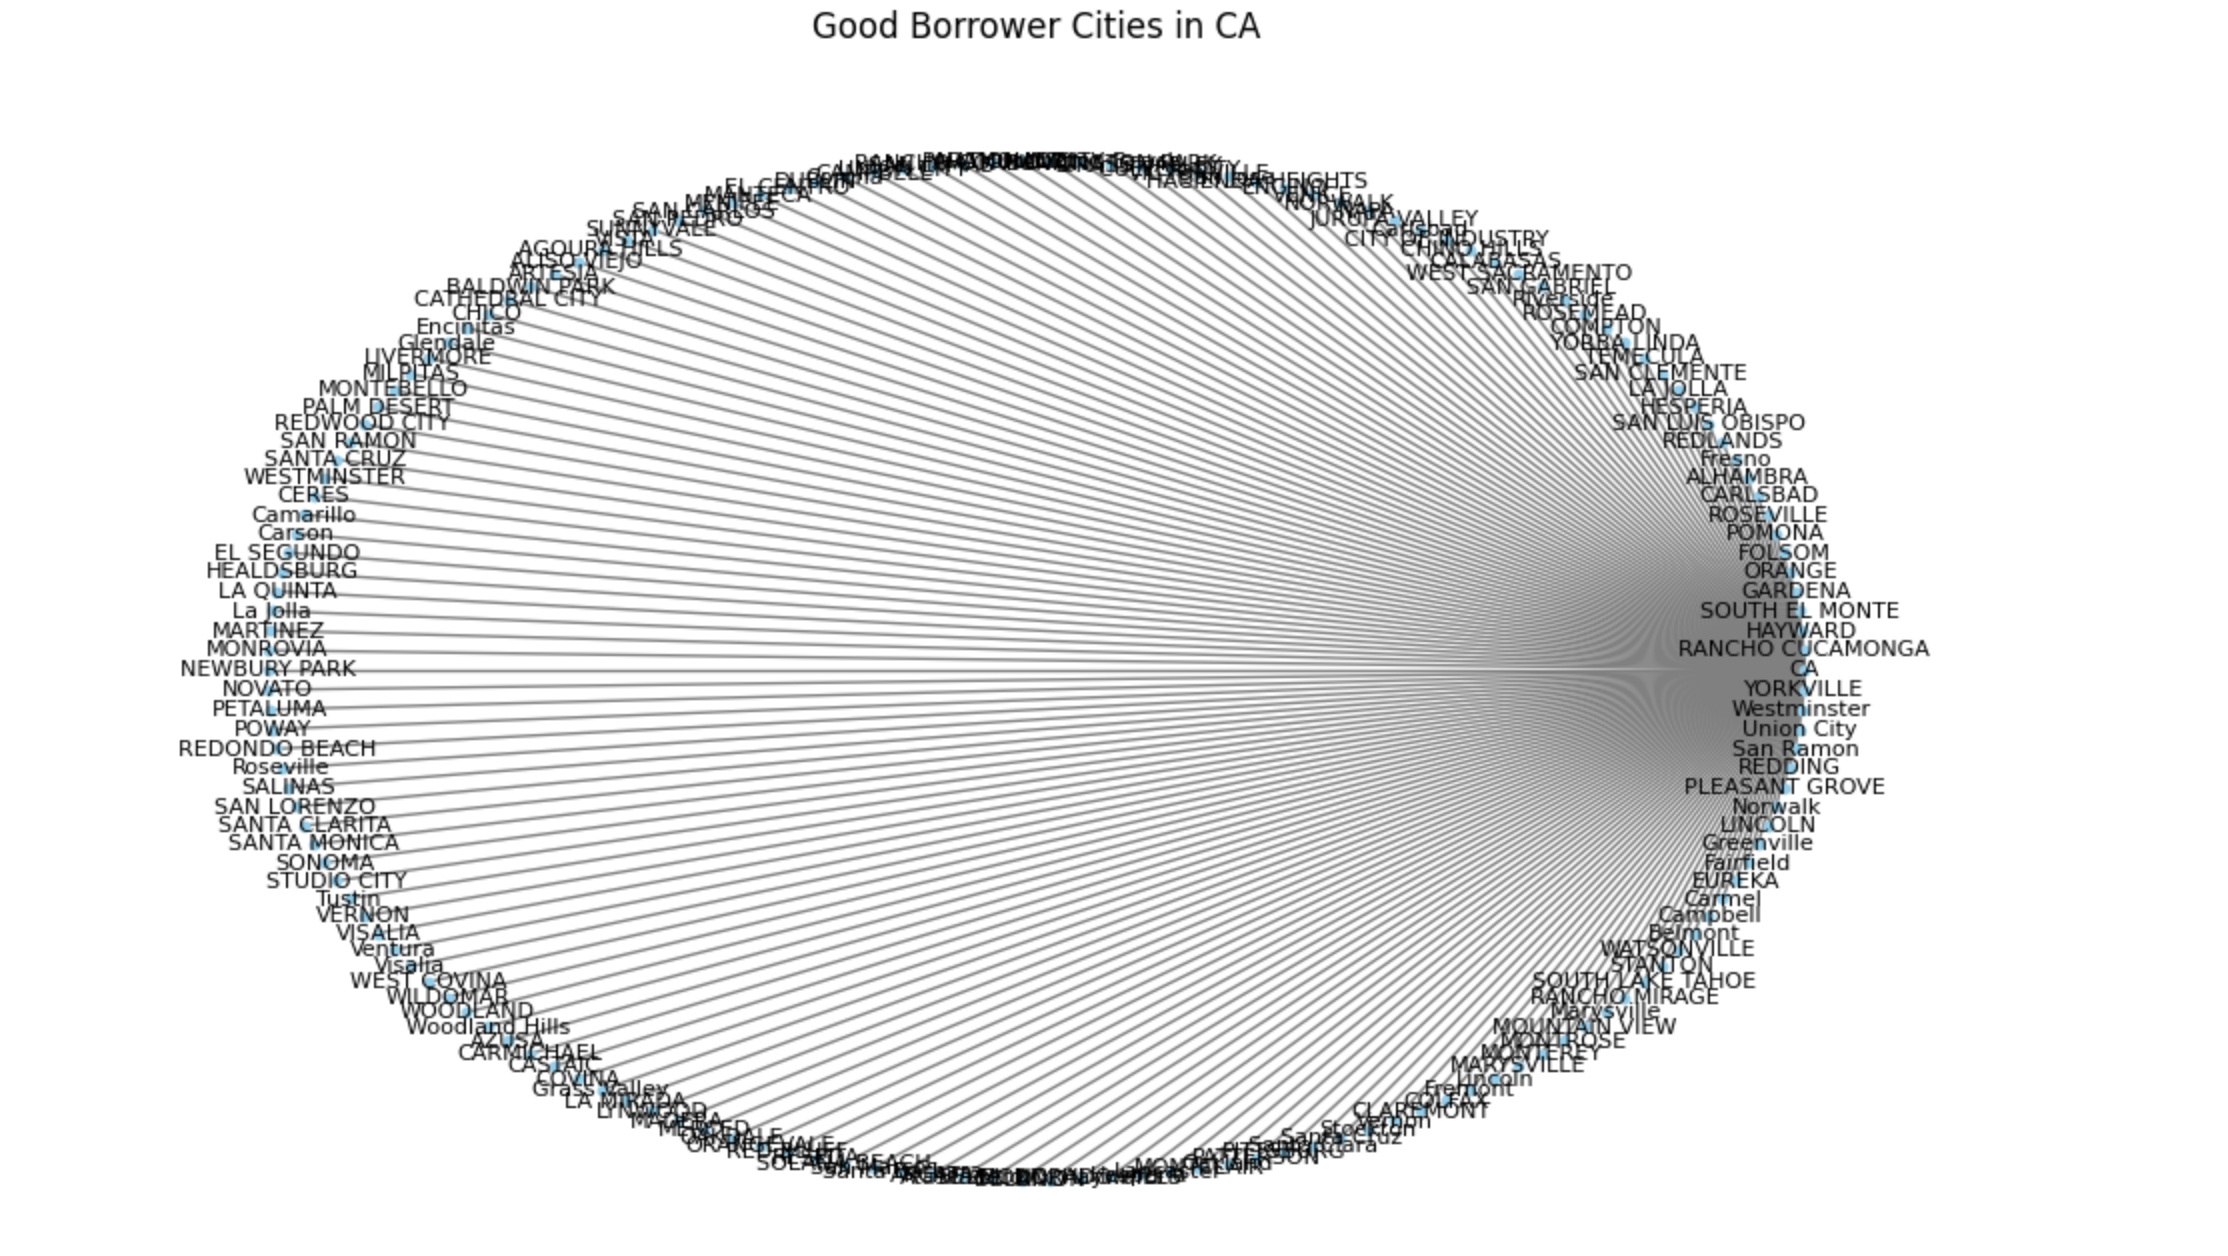
\includegraphics[scale=.3]{good_borrower_loans_7a.png}
\caption{Heterogeneity, Good Borrower Loans (limited to California)}
\end{figure}

For this example, I have a sketch of an idea that I hope to abstract away into a generic tool for creating graphs from relations. This is discussed in the next section.

\section{Creating a Graph from Relations, a Sketch of an Idea}

The input we get for tabular operational data is typically one of the following:
\begin{itemize}
\item One n-ary relation where all the $n$ entities in the relation are listed as a row in the table. Each row contains the $n$ identifiers for the $n$ entities, and the attributes associated with entities. This is the case for both the Olist and SBA examples.
\item Multiple relations from which we can construct a single n-ary relation. In other words, we can get a dataset $\mathbf{D} = \{ r_1, r_2, \ldots, r_m \}$ where each $r_i$ is a relation. Each relation $r_i$ has a set of entities and attributes associated with the entities. The relations can be used to construct a single n-ary relation $\mathbf{R} = \{ e_1, e_2, \ldots, e_n \}$ where each $e_i$ is an entity and the attributes associated with the entity are the attributes of the relation. This is the case when we want to learn a model that predicts an edge or a node in the graph. For now, we will assume that the input is a single n-ary relation $\mathbf{R}$, that is either given or can be constructed from the relations in $\mathbf{D}$.
\end{itemize}

We can then specify the entities and the relationships between the entities in the relation. This can be specified in a configuration file. The configuration file can be a simple YAML file that specifies the entities and the relationships between the entities. For example, an excerpt from the configuration file for the SBA example is shown below:

\begin{figure}[H]
\centering
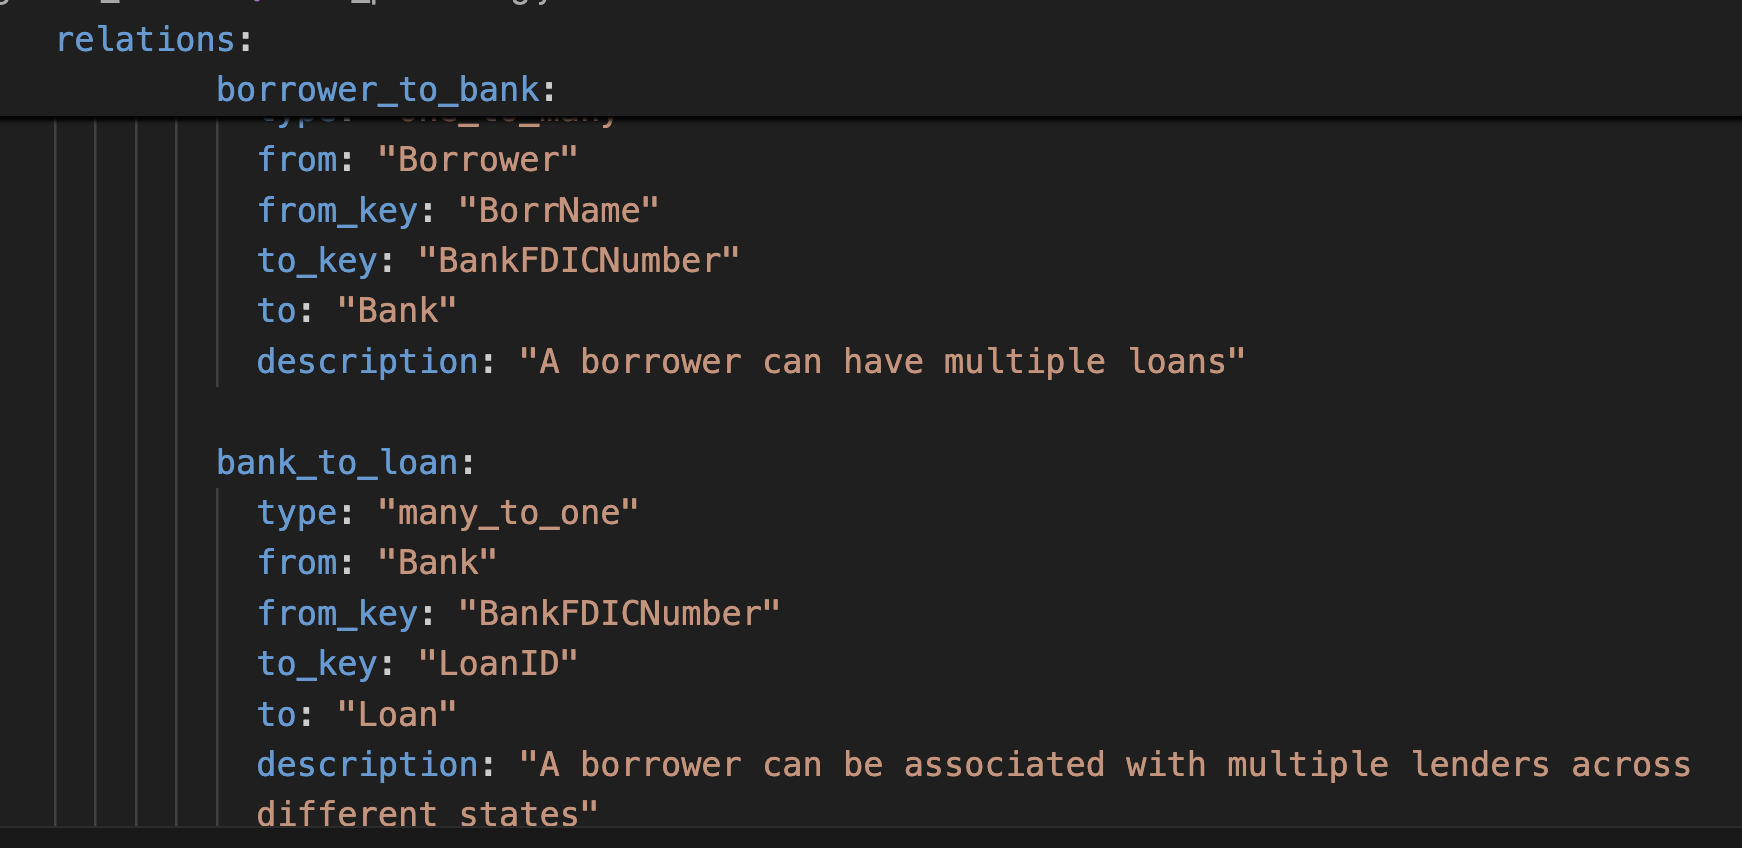
\includegraphics[scale=.35]{sba_graph_defn.png}
\caption{SBA Graph Definition}
\end{figure}

The graph derived from this definition is shown below.
\begin{figure}[H]
\centering
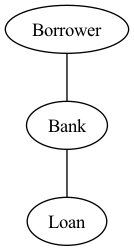
\includegraphics[scale=.35]{sba_7aloans_graph_schema.png}
\caption{SBA 7(a) Loans Graph Schema}
\end{figure}

So a possible approach to standardizing the process of creating a graph from relations is the following:
\begin{itemize}
\item Read the input data and construct a single n-ary relation $\mathbf{R}$.
\item Perform data cleaning and preprocessing on the relation $\mathbf{R}$.
\item Do the data analysis to identify the heterogeneity in the data.
\item Create a configuration file that specifies the entities and the relationships between the entities in the relation $\mathbf{R}$ for each subset of the data that is homogeneous with respect to the analysis or learning task.
\item Use the configuration file to create a graph from the relation $\mathbf{R}$.
\item Perform the analysis or learning task on the graph.
\end{itemize}

\section{Conclusion}
This is an initial draft of a process to analyze and learn from relational data that is heterogeneous in nature. The heterogeneity can be identified by using domain knowledge and data analysis techniques. The process of creating a graph from relations is a key step in this process. This is done using a simple configuration file. The examples provided illustrate how to create a graph from relations and how to identify heterogeneity in the relationships between entities. The next steps are to refine the process and to develop a generic tool for creating graphs from relations. Adding more rigor and examples to the process of identifying heterogeneity in different machine learning tasks is work in progress.

\bibliographystyle{plain}
\bibliography{references}

\end{document}